\documentclass[output=paper,hidelinks]{langscibook}
\ChapterDOI{10.5281/zenodo.13347666}
%\bibliography{localbibliography}

\author{Tabea Reiner\affiliation{LMU Munich}}
\title{Who needs posterior infinitives?}  
\abstract{In functional-typological as well as generative frameworks the notions of finiteness and tense have become more and more detached from each other over the past decades, especially if tense is understood in the broad sense of ``temporal relations''. Thus, temporally marked non-finites do not come as a surprise anymore. However, non-finites expressing anteriority seem to be much less surprising than non-finites expressing posteriority. Indeed, the latter appear to be considerably rarer than the former. Why should that be? The most straightforward version of a functional answer to this question seems to be: because we don’t need such forms. The present paper sets out to show that things are not that simple, drawing on an example from German.}

\IfFileExists{../localcommands.tex}{
  \addbibresource{../localbibliography.bib}
  \usepackage{tabularx,multicol}
\usepackage{url}
\urlstyle{same}

\usepackage{listings}
\lstset{basicstyle=\ttfamily,tabsize=2,breaklines=true}

\usepackage{langsci-optional}
\usepackage{langsci-lgr}
\usepackage{langsci-gb4e}
% \usepackage{langsci-textipa}

\usepackage{csquotes}
\usepackage{multirow}
\usepackage{colortbl}
\usepackage{ulem}
\usepackage{graphicx}
\usepackage{amsmath}
\usepackage{nicefrac}
\usepackage{tabto}
\usepackage{subcaption}
\usepackage{enumitem}
\usepackage{subcaption}


\usepackage{siunitx}
\sisetup{detect-weight=true, detect-family=true, detect-all, input-symbols={\%}, free-standing-units,group-digits=false,detect-inline-weight=math}

\usepackage[linguistics, edges]{forest}
\usetikzlibrary{matrix, arrows, arrows.meta}

\usepackage{pgfplots}
\usepgfplotslibrary{colorbrewer}
\pgfplotsset{cycle list/Dark2-4}

\usepackage{derivative}
\usepackage{langsci-branding}

  
\AtBeginDocument{%
  \SetupAffiliations{output in groups = false, 
                     separator between two = {\bigskip\\},
                     separator between multiple = {\bigskip\\},
                     separator between final two = {\bigskip\\}
                   }%
}

\newfontfamily\cjkfont
  [Scale=MatchLowercase]{SourceHanSerifSC-Regular.otf}
\AdditionalFontImprint{Source Han Serif}

\newcommand{\SC}{S\=uzh\=ou Chinese}
\newcommand{\MC}{Standard Chinese}
\newcommand{\THW}{T\`{a}ih\'{u} W\'{u}}
\newcommand{\SH}{Sh\`{a}ngh\v{a}i}
\newcommand{\iz}{ɨ̻}
\newcommand{\yz}{ʉ̻}
\newcommand{\zz}{ɿ}
\newcommand{\zw}{ʮ}
\newcommand{\pri}{*\textit{i}}
\newcommand{\pry}{*\textit{y}}
\newcommand{\prien}{*\textit{jen}}
\newcommand{\pryen}{*\textit{ɥɤn}}

\newcommand{\spr}[1]{\textsuperscript{#1}}

\renewcommand{\NG}{ŋ}
\newcommand{\textsubarch}{̯}
\renewcommand{\textschwa}{ə}
\renewcommand{\textprimstress}{ˈ}
\renewcommand{\textltailn}{ɲ}

\renewcommand{\textbabygamma}{\textramshorns}
\newcommand{\textramshorns}{ɤ}
\renewcommand{\textbardotlessj}{ɟ}
\renewcommand{\textbari}{ɨ}
\renewcommand{\textbeta}{β}
\renewcommand{\textctc}{ɕ}
\renewcommand{\textdyoghlig}{ʤ}
\newcommand{\textepsilon}{ɛ}
\renewcommand{\textesh}{ʃ}
\renewcommand{\textfishhookr}{ɾ}
\renewcommand{\textglotstop}{ʔ}
\renewcommand{\textlengthmark}{}
\renewcommand{\textopeno}{ɔ}
\newcommand{\textphi}{ɸ}
\renewcommand{\textrevepsilon}{ɜ}
\renewcommand{\textrtailr}{ɽ}
\renewcommand{\textrtailt}{ʈ}
\renewcommand{\textscriptg}{ɡ}
\renewcommand{\textthorn}{þ}
\renewcommand{\textturna}{ɐ}
\renewcommand{\textturnm}{ɯ}
\renewcommand{\textturnv}{ʌ}
\renewcommand{\textyogh}{ʒ}
\renewcommand{\textramshorns}{ɤ}
\renewcommand{\textbabygamma}{\textramshorns} %babygamma obsolete
\renewcommand{\textturnm}{ɯ}

\newcommand{\tone}[1]{\textsuperscript{#1}}
\newcommand{\underarch}{\textsubarch}

\newcommand{\sg}{\textsc{sg}}


\makeatletter
\let\thetitle\@title
\let\theauthor\@author
\makeatother


\newcommand{\togglepaper}[1][0]{
%   \bibliography{../localbibliography}
  \papernote{\scriptsize\normalfont
    \theauthor.
    \titleTemp ~
    To appear in:
    Dankmar W. Enke,   Larry M. Hyman,   Johanna Nichols,   Guido Seiler \&  Thilo Weber
    Language change for the worse.
    Berlin: Language Science Press. [preliminary page numbering]
  }
  \pagenumbering{roman}
  \setcounter{chapter}{#1}
  \addtocounter{chapter}{-1}
}


\newcommand{\ilit}[1]{#1\il{#1}}
  %% hyphenation points for line breaks
%% Normally, automatic hyphenation in LaTeX is very good
%% If a word is mis-hyphenated, add it to this file
%%
%% add information to TeX file before \begin{document} with:
%% %% hyphenation points for line breaks
%% Normally, automatic hyphenation in LaTeX is very good
%% If a word is mis-hyphenated, add it to this file
%%
%% add information to TeX file before \begin{document} with:
%% %% hyphenation points for line breaks
%% Normally, automatic hyphenation in LaTeX is very good
%% If a word is mis-hyphenated, add it to this file
%%
%% add information to TeX file before \begin{document} with:
%% \include{localhyphenation}
\hyphenation{
affri-ca-te
affri-ca-tes 
Scha-den
Zú-ñi-ga
Kaj-kwa-khrat-txi
}

\hyphenation{
affri-ca-te
affri-ca-tes 
Scha-den
Zú-ñi-ga
Kaj-kwa-khrat-txi
}

\hyphenation{
affri-ca-te
affri-ca-tes 
Scha-den
Zú-ñi-ga
Kaj-kwa-khrat-txi
}

  \togglepaper[6]
}{}


\begin{document}
\maketitle

\section{Introduction}\label{sec:reiner:1}
Traditionally, \textsc{finiteness} has been defined as a contingent property of verbs, viz. being marked for tense and person \citep[1]{Nikolaeva2007}. However, this definition has become more and more difficult to maintain in functional-typological as well as generative frameworks (cf. the recent overview by \citealt{Eide2016}). Proponents of the former were aware early on that neither tense nor person (or agreement, for that matter) were universal categories, which eventually resulted in a gradual notion of finiteness, pertaining to clauses (e.g., \citealt[852–864]{Givón1990}). Proponents of the latter departed from the tradition in making finiteness an essentially syntactic notion, hence also pertaining to clauses (e.g., \citealt{RitterWiltschko2014}). So across theories, tense and agreement have been downgraded to non-necessary ingredients of finiteness, the first of which will be focussed on in the present paper.

If finiteness can do without tense, then tense can do without finiteness. That is, we expect to find non-finites showing temporal marking – and indeed, we do. Consider examples \REF{ex:reiner:1} and \REF{ex:reiner:2}.

\ea\label{ex:reiner:1}Ancient Greek (Indo-European, \citealt[268]{Kavčič2016})\\
\gll ἅ φησι δρᾶσαι αὐτὸν Ἡσίοδος\\
what.\textsc{acc.pl} say.\textsc{3sg.pres} do.\textsc{aor.inf} him.\textsc{acc} Hesiod\\
\glt ‘what Hesiod says that he did’ (Plato, \textit{Republic} 377e8)\il{Ancient Greek}\il{Indo-European}
\ex\label{ex:reiner:2}Ancient Greek (Indo-European, \citealt[268]{Kavčič2016})\\
\gll ἐγὼ δ’ ἡγοῦμαι  βέλτιστα σε  πράξειν\\
I  but think.\textsc{1sg.pres} best.\textsc{adv} you.\textsc{acc}  do.\textsc{fut.inf}\\
\glt ‘But I think that you will do it best.’ (Isocrates 12.249)\il{Ancient Greek}\il{Indo-European}
\z

% % 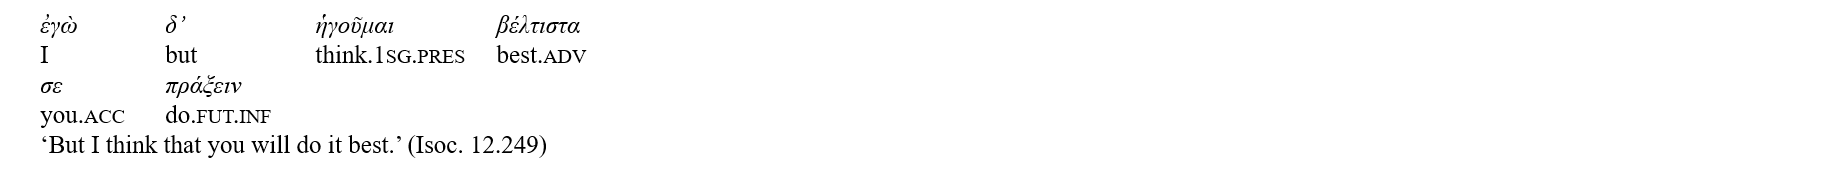
\includegraphics [scale=0.9] {figures/griechisch2.png}
% Bild \ili{Griechisch} 2

According to \citet[268]{Kavčič2016}, the infinitive in \REF{ex:reiner:1} refers to anteriority, where\-as the one in \REF{ex:reiner:2}  refers to posteriority. I interpret these terms in an adapted Kleinian framework (\citealt{Klein1994}, \citealt[305]{Reiner2019}) to mean the following:

\begin{description}
\item[Finite:]     	having a meaning with TSit and TT
\item[Non-finite:]     having a meaning with TSit but without TT 
\item[Infinitive:]     form having a meaning with TSit but without TT
\item[Anteriority:]	TSit before TX 
\item[Posteriority:]   TSit after TX,
\end{description}
where TSit is the time of situation, TT is the topic time (= time for which a claim is made), and TX is some specific time. Following Klein, I remain agnostic as to whether these times are spans or points. Crucially, TX may but need not coincide with either TU (time of utterance) or the matrix verb’s TT. In particular, the infinitival situation is not claimed to be real by the current speaker.

These terms can now be applied to example \REF{ex:reiner:1}. The infinitive’s TSit is located before TX and the latter presumably coincides with both TU and the matrix verb’s TT. Thus, the doing is before the time for which the current speaker claims the saying, but he does not claim the doing. Since the relation is ʻbeforeʼ (not: ʻextending toʼ) the example has been rendered by an \ili{English} simple past instead of a present perfect. Example \REF{ex:reiner:2} is analysed mirror-invertedly (here, the current speaker happens to quote himself, though).

In this sense, we are dealing with \textsc{temporal relations}. \il{Ancient Greek} is special in displaying both kinds of temporally marked infinitives (at least in indirect speech): anterior ones as well as posterior ones. Compare this to \ili{English}, where the structure of \REF{ex:reiner:1} might be mimicked by \REF{ex:reiner:3}, while the structure of \REF{ex:reiner:2} can hardly be replicated, as witnessed by \REF{ex:reiner:4}.

\ea[]{\label{ex:reiner:3}\itshape what Hesiod says to have done}
\ex[*]{\label{ex:reiner:4}\itshape But I consider you to will do it best.}
\z

This seems to be a very common situation in languages: there is something like an infinitive of anteriority, though arguably far from perfect, but no infinitive of posteriority. Is this impression accurate?

Starting from the (albeit arguable) assumption that infinitives of anteriority are indeed run-of-the-mill, I searched grammars specifically for infinitives of posteriority. In more detail, I went through a random subsample of the 318 languages in Velupillai's (\citeyear{Velupillai2016}) areally and genetically balanced sample. In each of her alphabetically ordered sections “[languages with] two tenses” and “[languages with] three tenses” I took the first five languages that had at least a past/future contrast and checked the corresponding sources for infinitives marking anteriority and posteriority, respectively. These languages were: \ili{Betoi}, \ili{Blackfoot}, \ili{Cavineña}, \ili{Chinantec/Lealao}, \ili{Ilocano} (each two tenses) and \ili{Aklan}, \ili{Akoye}, \ili{Alawa}, \ili{Albanian}, \ili{Ama} (each three tenses). In addition, I repeated the procedure for all languages in the section “[languages with] one tense”, where the source was readily available and that one tense was future.\footnote{Crucially, Velupillai’s definition of tense does not require markers to be obligatory, thus one-tense systems are possible \citep[94–95; 117]{Velupillai2016}. Otherwise, the absence of a marker (or its allomorphs) for tense value $x$ would imply absence of $x$ in the concept-to-be-expressed, hence establishing a two tense system with overtly marked $x$ and zero marked non-$x$ (also cf. \citealt[33–34]{Bybee1997}).} These languages were: \ili{Bao’an Tu}, \ili{Esselen}, \ili{West Greenlandic}, \ili{San Francisco del Mar Huave}, \ili{Javanese}, \ili{Kanamarí}, \ili{Koyra} \ili{Chiini}, \ili{Krongo}, \ili{Kunama}, \ili{Kuteb}, \ili{Navajo}, \ili{Nii}, \ili{Oneida}, \ili{Spokane}, \ili{Takelma}, \ili{Thai}. In order not to miss something obvious, I also included \ili{Livonian} \citep{Norvik2015} and \ili{Mari} \citep{Alhoniemi1993} as languages from the \ili{Finno-Ugric} family, whose members are quite famous for having “a rich non-finite verb system” \citep{RossHeeteTamm2010}. On similar grounds I added \ili{Turkish} with its diverse options for verbal embeddings \citep{Kornfilt2007} to my mini sample.

Thus, the mini sample consists of 29 languages and is consciously biased towards infinitives of posteriority. Since the latter were defined largely in a semantic way above (forms meaning ʻTSit after TXʼ, not involving TT), instances had often to be searched manually in the sources, i.e. by checking a great number of examples, usually far beyond the pages given by Velupillai. As heuristic strategies, I excluded forms with consistently more-than-temporal meanings (\citealt[10]{Dahl1985}, \citealt[23]{Dahl1985}) as well as forms embedded directly below complementiser-like elements, which I treated as an indication for TT (following \citealt[219–220]{Klein1994}). Moreover, I had to rely heavily on glosses and translations.

As a result, five candidates for infinitives of posteriority remained, most of which, however, come with certain problems to be explained below.

Maybe the most obvious candidate is from \ili{Turkish}, which seems to replicate almost exactly the \ili{Ancient Greek} structure:

\ea\label{ex:reiner:5} Turkish (Turkic, \citealt[312]{Kornfilt2007})\\
\gll {[Sen-i}		    {sınav-ı}	            {geç-ti]}         {san-ıyor-um}\\
 you-\textsc{acc} test-\textsc{acc} pass-\textsc{pst}	believe-\textsc{prspr}-\textsc{1sg}\\    
\glt ʻI believe you to have passed the test.ʼ\il{Turkish}\il{Turkic}\\
\ex\label{ex:reiner:6} Turkish (Turkic, \citealt[312]{Kornfilt2007}) \\
\gll {[Seni-i}		{sınav-ı}	{geç-ecek]}   {san-ıyor-um}\\
    you-\textsc{acc} test-\textsc{acc}	pass-\textsc{fut}    believe-\textsc{prspr}-\textsc{1sg}\\
\glt ʻI believe you to pass the test (in the future).ʼ\il{Turkish}\il{Turkic}
\z

In \REF{ex:reiner:6}, the addressee’s passing of the test appears not to be claimed directly (hence no TT) but it is situated after some specific time (hence TSit after TX). The absence of TT becomes even clearer in the following example.

\ea\label{ex:reiner:7} Turkish (Turkic, \citealt[557]{Kornfilt2018}) \\
\gll {Herkes}		{[ben-i}		{üniversite-ye}   {başla-yacak]}	{san-ıyor}\\
    everybody	I-\textsc{acc}		university-\textsc{dat}  start-\textsc{fut}	believe-\textsc{prspr}\\
\glt ʻEverybody believes me to be starting university.ʼ\il{Turkish}\il{Turkic}\\
\z

Please note that according to the largely semantic definitions used here it does not matter whether or not our examples involve the \ili{Turkish} infinitive suffix \emph{\hbox{-}mAK} \citep[392]{Kornfilt1997}, as long as the forms (\emph{geç-ecek} and \emph{başla-yacak}) convey the relevant meaning. In sum, \ili{Turkish} seems to provide unambiguous and unproblematic examples for infinitives of posteriority.
Next, consider \ili{Thai}:\largerpage[-1]

\ea\label{ex:reiner:8} \ili{Thai} (Tai, \citealt[772]{Hudak1987}, \citealt[692]{Hudak2018})  \\
\gll {phǒm}	{mây}	{yàak}		{cà	rian}	{wíchaa}	{nán}\\
I		not	want.to	will	study	subject	that  \\ 
\glt ʻI don’t want to study that subject.ʼ  \\ 
\z  

Semantically, this example appears to be as clear as the \ili{Turkish} ones: the studying is not claimed to be the case (no TT) but situated after some specific time (TSit after TX). Formally, however, one may dispute whether \emph{cà rian} should count as one form (hence being able to meet the definition of infinitive given above).
A similar problem holds for \ili{Koyra} \ili{Chiini}:

\ea\label{ex:reiner:9} Koyra Chiini (Nilo-Saharan, Mali; \citealt[164]{Heath1999})\\ 
\gll {a}		{yee-kate}		{ka}	{ta}	{filla}   {[ŋgu}		{goy}		{di]}\\
\textsc{3.sg.s}    return-\textsc{centrip}  \textsc{inf} \textsc{fut} repeat  \textsc{3.refl.sg}	work    \textsc{def}\\
% im mail schauen, was sich worauf bezieht
\glt ‘He has come back to repeat (=continue) his work.’\il{Koyra Chiini}\il{Nilo-Saharan}\\
\z  

Moreover, \emph{ka ta} is not only non-obligatory \citep[163]{Heath1999} – which is compatible with the definitions used here – but “fairly rare” \citep[164]{Heath1999}. In fact, \citet[311]{Heath1999} gives various parallel examples without \emph{ta} (numbers 592c, d, g there). Likewise, \emph{ta} can, but not always does, mark pure posteriority (or future, which I take to be posteriority relative to TU): it is also associated with “diffuse potentiality” as well as “irrealis” \citep[163]{Heath1999}. So, in addition to sparse attestation, the question remains which meaning is at stake in example \REF{ex:reiner:9}.
Maybe the most intricate examples for a potential infinitive of posteriority come from \ili{West Greenlandic}:


\ea\label{ex:reiner:10} West Greenlandic (Eskimo-Aleut, \citealt[276]{Fortescue1984})\footnote{The contemporative mood seems to mark converbphrases (cf. \citealt[3]{Haspelmath1995}). So a more (but not quite) literal translation of the first example could be: ʻHe hesitated before his approaching herʼ.}\il{West Greenlandic}\il{Eskimo-Aleut}\\
 
\gll {palli-ssa-llu-gu}				{nangaa-vu-q}\\
approach-\textsc{fut-ct-3sg.o.ct}		hesitate-\textsc{intr}-\textsc{3sg}\\
\glt ‘He hesitated to approach her.’ \\
\ex\label{ex:reiner:11} West Greenlandic (Eskimo-Aleut, \citealt[276]{Fortescue1984}) \\
\gll    niriursui-vu-nga    aqagu		urni-ssa-llu-tit \\
        promise-\textsc{intr}-\textsc{1sg} tomorrow	come\_to.\textsc{fut-ct-2sg.o.ct}\\
\glt    ‘I promise to come to you tomorrow.’\il{West Greenlandic}\il{Eskimo-Aleut}\\
\z 

The relevant meaning (TSit after TX, no TT) seems to be present and \emph{palli-ssa-llu-gu}\slash\emph{urni-ssa-llu-tit} are generally considered word forms (but cf. \citealt{Haspelmath2018}). Neither is it a problem that the CT-forms are not infinitives in a more traditional sense than the one chosen here. However, there is no consensus that \emph{-ssa-} as such actually expresses anything temporal at all (\citealt{Bittner2005}).

As a last candidate for an infinitive of posteriority consider an example from \ili{Nii}:

\ea\label{ex:reiner:12} Nii (Trans New Guinea, PNG, \citealt[80]{StuckyStucky1976})\\
\gll {si-mba}		{e-ner-im}\\
    take-\textsc{3.fut}	do-\textsc{neg-3.compl}\\
\glt ‘He is not about to take (it).’\il{Nii}\il{Trans New Guinea}\\
\z 

By all criteria this seems to be a pertinent example; however, \citet{StuckyStucky1976} give considerably less semantic information than for example Heath, so I do not dare draw any definite conclusions.
In total, I take the yield from my mini sample to be sufficiently poor to uphold the hypothesis that infinitives of posteriority are much rarer than are infinitives of anteriority.

Still, another strategy for identifying languages with an infinitive of posteriority might consist in picking retrospective languages in the sense of \citet{Ultan1978}~– possibly, for those languages, the picture is reversed and we find hardly any infinitives of anteriority but good candidates for infinitives of posteriority. However, the random sample above already includes at least three potentially retrospective languages (\ili{Aklan}, \ili{Blackfoot}, \ili{Spokane} – if not all languages with only future tense) and those mentioned by \citet{Ultan1978} also seem to lack infinitives of posteriority, maybe partly due to not having infinitives in any sense at all: Dakota (\citealt[105, 156]{BoasDeloria1976})\footnote{Admittedly, there is relative tense; however, provided that relative tense involves TT (not just TSit and TX), it is fundamentally different from temporally marked infinitives as defined here. The same holds for \ili{Rotuman} \citep[23]{Churchward1940}.}, \ili{Guaraní} (\citealt{GregoresSuárez1967}), \ili{Hopi} (\citealt{Masayesva-Jeanne1978}, \citealt{HillBlack1998}), \ili{Onondaga} (\citealt{Barrie2015}, \citealt{Woodbury2018}), \ili{Rotuman} (\citealt{Churchward1940}), and \ili{Tairora} (\citealt[esp. p. 577]{Vincent1973}, \citealt{McKaughan1973}).

In view of all the data presented so far, I stick with the view that infinitives of posteriority are scarce in comparison to infinitives of anteriority. However, a more comprehensive survey on these phenomena definitely constitutes a desideratum.

As an aside, the asymmetry might be accompanied by a second one, i.e. one between infinitives of posteriority and future tenses: the latter abound, judging from \citet{Velupillai2016}. However, there is a risk that Velupillai’s results have been skewed by the peculiarities of grammar writing: authors tend to distinguish very carefully past tenses from various aspects, whereas futures are rarely separated from prospective aspects (another danger to the candidates presented above). Thus, a number of futures in the survey might not be futures after all, for example in \ili{Kunama} as documented by \citet{Böhm1984}.\footnote{To be sure, the distinction between future and modality is taken very seriously by \citet[101]{Velupillai2016}.} Therefore, I will ignore the second (potential) asymmetry and focus on the first one: there appear to be many more languages and many more contexts that allow infinitives of anteriority than of posteriority.

This asymmetry requires an explanation. Perhaps the most obvious one is a directly functional hypothesis: in most infinitival constructions, speakers need to mark anteriority rather than posteriority, since the latter is mostly given from context. However, directly functional explanations can run into problems, for example compare the following two quotations from \citet{Schmidtke-Bode2009} on temporal and modal markings in purpose clauses.

\begin{quote}
“The fact that the majority of purpose clauses come as deranked constructions and are hence often deprived of tense-aspect marking has a fairly straightforward explanation. It is part of the conceptual structure of purposive situations ([...]) that \emph{purposes are intrinsically future-oriented}. In linguistic terms, purpose clauses inherently have what Noonan (1985:92) calls ‘determined time reference’ in relation to the matrix clause situation. \emph{Consequently, there is no strict communicative need to overtly specify the temporal location of the purposive situation}. We find here a classic case of economical behaviour rooted in the predictability of information in discourse. Speakers can afford to omit overt temporal information, thus being able to make an economical choice for a shorter, less overtly marked non-finite purpose clause construction (cf. also Jespersen 1924 or Haiman 1983 for the general idea). This motivates the cases in which tense-aspect marking is absent from a purposive construction. As Givón notes, ʻthe more predictable—i.e. continuous, coherent, non-switching—a clausal feature is vis-à-vis its immediate inter-clausal context, the more likely it is to be left unmarked—i.e. less finiteʼ (Givón 1991: 876), [...].” (\citealt[42–43]{Schmidtke-Bode2009}, my emphasis)

“More generally, \emph{overt mood marking in purpose clauses does certainly not come as a great surprise. Purposive situations are inherently modal} in a two-fold way. On the one hand, they are necessarily hypothetical because the outcome of a purposeful action is yet to be achieved, i.e. non-realized at the moment of speech. As Hewitt (1987:40) aptly puts it, ʻ[a]s the accomplishment of any intention may be foiled as events unfold, it is clearly appropriate if a language should choose to have recourse to a non-factual mood for the representation of purpose.ʼ On the other hand, Palmer (1986:174) points out that purposes by their very nature contain a desiderative element, since they refer to someone’s intention to realize a certain goal or to make a certain situation obtain in the future.” (\citealt[45]{Schmidtke-Bode2009}, my emphasis)
\end{quote}

Thus, purpose clauses commonly (i) do not receive temporal marking, since they are inherently future-oriented and (ii) do receive modal marking, since they are inherently hypothetical-desiderative. Put in other words, one category \emph{is not} overtly marked because it is already given, while another category \emph{is} overtly marked because it is already given. So one and the same factor carries the burden of explaining two opposing outcomes.

Transferring this to infinitives of posteriority, even if we can prove that in most cases posteriority (but not anteriority) is given from context in infinitival constructions, we still have to choose between two predictions: posteriority will be marked simply because it is given or posteriority will not be marked precisely because it is already given. One might object that in contrast to the arguments quoted above, posteriority in infinitival constructions is not an \emph{inherently} given property (at least not in all cases; obviously there is an overlap between infinitival constructions and purpose clauses). However, as far as I can see, nothing in those arguments hinges on the property being inherent. As an interim summary, the directly functional hypothesis (“in most infinitival constructions, speakers rather need to mark anteriority than posteriority, since the latter is mostly given from context”) can explain both the asymmetry we find (“don’t mark the obvious”) \emph{and} a hypothetical situation where posteriority as well as anteriority is regularly marked after all (“do mark the obvious”). However, an explanation that does not only account for the explanandum but also for its opposite does not appear very convincing.

There are two ways out of this, which presumably have to be combined: focussing on diachrony and focussing on (synchronic) systems as a whole. Both bring in additional factors and interaction among these factors, even including dysfunctional analogies (\citealt[161–164]{Newmeyer1998}, \citealt{Seiler2015}, \citealt[3]{CristofaroZúñiga2018}). Crucially, this means that certain phenomena in isolation might be very hard to motivate by functional factors like expressive power or speaker/hearer economy. Examples from \ili{German} are given by \citet[246]{Seiler2015}, for instance the requirement that the prefield position be filled by exactly one constituent – despite the fact that this position is used for topicalisation and speakers might want to topicalise information that is encoded in more than one constituent. For any such phenomenon, the challenge is motivating it anyhow by taking into account its syntagmatic, paradigmatic, and historical connections.

Thus, the asymmetry between infinitives of anteriority and infinitives of posteriority might receive a more complex but still functional account, even if the few existing infinitives of posteriority should prove completely useless in isolation. In the present contribution I do not intend to give such a full account but confine myself to scrutinising a sixth candidate for an infinitive of posteriority, which is (right headed) [\textsc{inf} [\emph{zu} \textit{werden}\textsubscript{INF}] from \ili{German} (cf. \sectref{sec:reiner:2.1}, \sectref{sec:reiner:2.2}). I will argue that this structure as such is hard to motivate functionally even from a diachronic perspective and hence may be the result of analogy for analogy’s sake (\sectref{sec:reiner:2.3}). If this analysis is on the right track, we are dealing with a local but not necessarily global change for the worse.

\section{Case study: [\textsc{inf} [(\emph{zu}) \textit{werden}\textsubscript{INF}]] in German}\label{sec:reiner:2}

\subsection{The phenomenon: An infinitive of posteriority in German}\label{sec:reiner:2.1}\largerpage[2]

As might be expected from the small survey in \sectref{sec:reiner:1}, the sixth candidate for an infinitive of posteriority, i.e. the one from \ili{German}, is not an entirely clear case either. I will deal with the problems in \sectref{sec:reiner:2.2}, after presenting the structure as such in the current section. For ease of exposition I will switch back and forth between the terms \emph{infinitive of posteriority} and \emph{posterior infinitive} with no difference in meaning intended (accordingly for \emph{infinitive of anteriority} and \emph{anterior infinitive}).

The \ili{German} infinitive of posteriority can be demonstrated best by way of constructed examples, later followed by real ones. To begin with, consider the finite source structure, first, in an independent clause \REF{ex:reiner:13}, then in a subordinate clause \REF{ex:reiner:14}. The first example is finite in every possible way, the second one is less so for the very reason that it is subordinated (cf. Givón's \citeyear{Givón1990} notion of finiteness as [–integration]). Conveniently enough, this difference does not play a role using the definitions from \sectref{sec:reiner:1}.


\ea\label{ex:reiner:13} German (Indo-European) \\
\gll    {Er}	{wird}		{schlaf-en.}\\
he	will.\textsc{3sg}	sleep-\textsc{inf}\\
\glt ‘He will be sleeping.ʼ\\
non-posterior meaning: ʻProbably, he is sleeping (right now).ʼ \\
posterior meaning: ʻHe will be sleeping.ʼ\il{German}\il{Indo-European}\\
\ex\label{ex:reiner:14} German (Indo-European)\footnote{This use might be restricted (\citealt[195–196]{Wilmanns1906}, \citealt[230]{Gelhaus1975}) or not \citep[27]{Hilpert2008}; in any case it is possible in principle.}\\
\gll  {\dots dass}	{er}	{schlaf-en}	{wird.}\\
that	he	sleep-\textsc{inf}	will.\textsc{3sg}\\
\glt  ‘\dots that he will be sleeping.’ \\
non-posterior meaning: ‘\dots that probably he is sleeping (right now).’ \\
posterior meaning ‘\dots that he will be sleeping.’\il{German}\il{Indo-European}\\
\z

Now, consider the non-finite version of each example, given in \REF{ex:reiner:15} and \REF{ex:reiner:16}, respectively.


\ea\label{ex:reiner:15} German (Indo-European) \\
\gll    {\dots dass}	{er}	{schlaf-en}	{werd-en}	{muss.}\\
        that	he	sleep-\textsc{inf}	will-\textsc{inf}	can \\
\glt    possible meaning: ‘\dots that he must [sleep in the future].’\il{German} \il{Indo-European}\\
\ex\label{ex:reiner:16} German (Indo-European) \\
\gll    {Er}	{hofft,}		{schlaf-en}	{zu}	{werd-en.}\\
        he	hope.\textsc{3sg}	sleep-\textsc{inf} \textsc{part}	will-\textsc{inf}\\
\glt possible meaning: ‘He hopes [to sleep in the future].’\il{German}\il{Indo-European}\\
\z

Both the bare infinitive \emph{schlafen werden}  in \REF{ex:reiner:15} as well as the particle infinitive \emph{schlafen zu werden} in \REF{ex:reiner:16} appear to fulfil the definition of posterior infinitives given in \sectref{sec:reiner:1} above (TSit after TX, no TT). Furthermore, the particle infinitive can have characteristics of an inherently embedded clausal structure of its own, while the bare one cannot; rather it forms one clause with its higher predicate, here \emph{muss} (\citealt{RappWöllstein2013}). Note that in the example at hand this clause is itself an embedded one. So the question arises for \REF{ex:reiner:15} but not for \REF{ex:reiner:16} whether the immediate clausal environment of the posterior infinitive may also be an independent clause. Such examples can easily be constructed, cf. \REF{ex:reiner:17}.

\ea\label{ex:reiner:17} German (Indo-European) \\
\gll    {Er}	{muss}		{schlaf-en}	{werd-en.}\\
     he	must.\textsc{3sg}	sleep-\textsc{inf}	will-\textsc{inf}\\
\glt    possible meaning: ʻHe must [sleep in the future].ʼ\il{German}\il{Indo-European}\\
\z 

However, for practical reasons laid out in \citet{Reiner2018} I leave aside this type. Likewise, the issue of entirely independent infinitives \citep{Fries1983}, including the question whether those should be called \emph{infinitives} at all, is not covered here.
Thus, the central patterns for the purposes of this paper are the ones exemplified in \REF{ex:reiner:15} and \REF{ex:reiner:16}, which may be generalised as right-headed [\textsc{inf} [\emph{zu} \textit{werden}\textsubscript{INF}]]. Just before turning to real examples for this structure and addressing those examples’ properties, I would like to contrast the infinitive of posteriority with its anterior counterpart, i.e. right headed [\textsc{pstptcp} [\emph{(zu) haben/sein}]], shown below with \emph{haben}. Again, the bare infinitive is presented first, then the particle infinitive.\largerpage[1]

\ea\label{ex:reiner:18} German (Indo-European)\footnote{Depending on co(n)text, an epistemic reading of the embedding modal might be preferred.}\\
\gll {\dots dass}	{er}	{geschlafen}		{hab-en}	{muss.}\\
 that	he	sleep.\textsc{pstptcp}	have-\textsc{inf}	must.\textsc{3sg}\\
\glt    ʻ\dots that he needs to have slept [e.g., before going to work].ʼ\il{German}\il{Indo-European}\\
\ex\label{ex:reiner:19} German (Indo-European) \\
\gll    {Er}	{behauptet}	{geschlafen}		{zu}	{hab-en.}\\
    he	claims		sleep.\textsc{pstptcp}	\textsc{part}	have-\textsc{inf}\\
\glt ʻHe claims to have slept.ʼ\il{German}\il{Indo-European}\\
\z 

In parallel to posterior infinitives, the sleeping is not claimed (at least not directly, in \REF{ex:reiner:19} the matrix predicate adds this meaning), hence no TT is conveyed by the form. Likewise, TSit is located before some specific time, hence TSit before TX. Please note that the semantics described here might count as aspectual in other frameworks (cf. \citealt[116–117]{Abraham2004}).

In contrast to posterior infinitives (see below), anterior infinitives are considered part of the standard inventory of \ili{Standard German} (cf., e.g., \citealt[2159–2160]{ZifonunStrecker1997}). As such, they are presumably known to speakers (even if they are not used extensively in everyday speech) and might act as a model in analogy, which will become important in \sectref{sec:reiner:2.3}.

After presenting the structure of the posterior infinitive as well as of its anterior counterpart both by means of constructed examples, some real examples are in order. These come from an extensive corpus study within the DeReKo (sub-corpus \textsc{tagged-c-}öffentlich) where, as a result, 267 instances of the bare version were found and four of the particle version (a discrepancy to be discussed in \sectref{sec:reiner:2.2}). Details of this study can be found in \citet{Reiner2018}; let me just note here that all examples have been checked manually and that both numbers (267 as well as four) outrank the numbers for comparable slips of the pen, which had been searched for comparison.

First, consider some examples for the bare infinitive of posteriority. They are sorted according to (i) general type of finite embedding verb (modal vs. auxiliary), (ii) aktionsart type of the most deeply embedded (i.e. lexical) infinitive, (iii) [+/\textminus{}] indication of posterior meaning from context, in particular via temporal adverbials, (iv) selected syntactic characteristics.

\begin{enumerate}[label=(\roman*)]
\item Of the 267 finite embedding verbs, 250 were modals: \emph{können}~ʻcanʼ (136), \emph{müssen}~ʻmustʼ (96), \emph{sollen}~ʻshouldʼ (8), \emph{dürfen}~ʻmayʼ (6), \emph{wollen}~ʻwant toʼ (3), \emph{mögen}~ʻlike toʼ (1) and 16 were auxiliaries: conditional \emph{werden}, i.e. \emph{würd-} (3), for forming various periphrases (e.g., the future-in-the-past) and finally future \emph{werden} itself (13). The occurrence of the latter was expected in light of Rothstein’s works on double futures (\citealt{Rothstein2012}, \citealt{Rothstein2013a}, \citealt{Rothstein2013b}). 

The one remaining matrix verb is \emph{haben} ʻhaveʼ, only appearing in one peculiar example. Here is a typical example with \emph{können} as the finite verb (\emph{könne}):


\ea\label{ex:reiner:20} \ili{German} (\ili{Indo-European}) \\
\gll    {Er}	{rechne}	{allerdings}	{damit,} {dass}	{Scharon}	{wieder}	{sprech-en}   {und}	{versteh-en}		{werd-en}	{könne.}\\
he	expects	though	on.this that	Sharon	again		speak-\textsc{inf}   and	comprehend-\textsc{inf}	will-\textsc{inf}	can \\ 
\glt    ‘He expects that Sharon will be able to speak and comprehend again.’ (lit.: can will comprehend) \\
\z 

Next is an example with \emph{würd-} as the finite verb, as a whole representing a future-in-the-past:



\ea\label{ex:reiner:21} 	\ili{German} (\ili{Indo-European}, Niederösterreichische Nachrichten, 22 January 2007) \\
\gll {Geprägt}		{von}	{guten}	{Aktionen}	{beider}	{Mannschaften,}		{war}		{lange}		{Zeit}    {nicht}	{ersichtlich,}	{wer}	{sich}	{schlussendlich}  {durchsetz-en}	{werd-en}	{würde.}\\
characterised	by	good	moves		of.both teams			was		long		time not	obvious	who	\textsc{refl}	eventually   prevail-\textsc{inf}	will-\textsc{inf}	will.\textsc{3sg}.\textsc{cond}\\
\glt ʻCharacterized by good moves of both teams, it was not clear for a long time who would eventually prevail.ʼ (lit.: would will prevail)  \\
\z 

And, to conclude segment (i), here is another example from the sports pages, showing future \emph{werden} itself as the finite verb (\emph{wird}):

\ea\label{ex:reiner:22} 	\ili{German} (\ili{Indo-European}, Niederösterreichische Nachrichten, 21 May 2008) \\
\gll    {Inwieweit} {sich}	{Tamara}	{im}	{Finale}  {behaupt-en}			{werd-en}	{wird,}   {werden}		{dann}		{wieder}	{Nuancen} {entscheiden,}	{denn}	{dort}		{warten}  {schon}		{weitere}	{Riesentalente}  {auf}	{die}	{Finalentscheidung.}\\
to.what.extent		\textsc{refl}	Tamara	in.the	final   hold.one’s.own-\textsc{inf}		will-\textsc{inf}	will.\textsc{3sg}    will		then		again		nuances decide		for	there		wait    already		other		giant.talents   for	the	final.decision \\
\glt ʻThe extent to which Tamara will hold her own in the final will then be decided by nuances again, as there will already be other giant talents waiting for the final decision.ʼ (lit.: will will hold her own) \\
\z 

\item As to the aktionsart type of the most deeply embedded (i.e. lexical) infinitive, no tendency towards either atelic or telic verbs could be noted. Below is one example for each type, atelic (\emph{konkurrieren}) in \REF{ex:reiner:23} and telic (\emph{aufnehmen}) in \REF{ex:reiner:24}.



\ea\label{ex:reiner:23} 	\ili{German} (\ili{Indo-European}, Nürnberger Zeitung, 21 March 2007) \\
\gll    {Er} {wies} {darauf} {hin,}	{dass}	{die}	{Bundeswehr}  {angesichts}	{der}	{bevorstehenden}  {geburtenschwachen}	{Jahrgänge}	{etwa}    {ab}		{2008}		{zunehmend}   {mit}	{der}	{Wirtschaft}	{um}	{Arbeitskräfte}   {konkurrier-en}		{werd-en}	{müsse.}\\
he	pointed.out    {} {}	that	the	\emph{Bundeswehr}  in.view.of	the	imminent    low-birthrate		years		ca. from.on		2008		increasingly    with	the	economy	for	workers compete-\textsc{inf}		will-\textsc{inf}	must.\textsc{3sg}.\textsc{quot}\\
\glt ʻHe pointed out that the Bundeswehr [German armed forces] would have to compete increasingly with private enterprises for workers from 2008 onwards in view of the low birth rates in that age group.ʼ (lit.: must will compete)
\ex\label{ex:reiner:24} 	\ili{German} (\ili{Indo-European}, St. Galler Tagblatt, 20 March 2000) \\
\gll    {In}		{einem}		{Schlussvotum}	{verlieh} {Alex}	{Thalmann,}	{Präsident}	{der} {Museumsgesellschaft}		{Bischofszell,}		{seiner}  {Hoffnung}	{Ausdruck,}	{dass}	{in}	{naher}	{Zukunft} {ein}	{Kulturbeauftragter}		{sein}	{Amt}	{in}  {Bischofszell}	{aufnehm-en}	{werd-en}	{kann.}\\
in		a		final.vote		gave    Alex	Thalmann	President	of.the  Museumsgesellschaft		Bischofszell		his hope		expression	that	in	near	future  a		cultural.commissioner	his	office	in  Bischofszell	take.up-\textsc{inf}	will-\textsc{inf}	can.\textsc{3sg}\\
\glt  ʻIn a final vote Alex Thalmann, President of the Museumsgesellschaft Bischofszell [Municipal Society for Museums], expressed his hope that in the near future a cultural commissioner could take up his office in Bischofszell.ʼ (lit.: can will take up) 
\z 

More generally, only a few lexemes occurred more often than once as the infinitive in [\textsc{inf} \textit{werden}\textsubscript{INF}]. These were:

\begin{sloppypar}
\emph{absagen}  ʻcancelʼ (2), \emph{antreten}  ʻcompeteʼ (3), \emph{aufbringen}  ʻraise (funds)ʼ (2), \emph{auskommen}  ʻget by (financially)ʼ (3), \emph{beginnen}  ʻstartʼ (2), \emph{bewältigen}  ʻovercomeʼ (2), \emph{bezahlen}  ʻpayʼ (3), \emph{entscheiden}  ʻdecideʼ (2), \emph{erfüllen}  ʻfulfilʼ (3), \emph{fahren}  ʻrideʼ (2), \emph{genießen}  ʻenjoyʼ (3), \emph{gestalten}  ʻshapeʼ (2), \emph{halten}  ʻkeepʼ (10), \emph{hinnehmen}  ʻput up withʼ (3), \emph{in Anspruch nehmen} ʻuse/begin usingʼ (3), \emph{investieren in}  ʻinvestʼ (2), \emph{konkurrieren}  ʻcompeteʼ (3), \emph{Kredit aufnehmen} ʻborrow (money)ʼ (2), \emph{lassen}  ʻletʼ (2), \emph{leben mit}  ʻcope withʼ (3), \emph{mitspielen}  ʻplay (with others)ʼ (2), \emph{nutzen}  ʻuseʼ (2), \emph{präsentieren}  ʻpresentʼ (2), \emph{sehen}  ʻseeʼ (2), \emph{sich befassen mit}  ʻconcern oneself withʼ (2), \emph{sich durchringen zu}  ʻbring oneself to do sth.ʼ (2), \emph{sich einigen} 'agree' (2), \emph{sich leisten}  ʻaffordʼ (10), \emph{sich verabschieden}  ʻsay goodbyeʼ (2), \emph{sprechen und verstehen}  ʻspeak and comprehendʼ (3), \emph{tun}  ʻdoʼ (2), \emph{über die Bühne gehen}  ʻgo smoothlyʼ (2), \emph{übernehmen}  ʻtake over (e.g., expenses)ʼ (3), \emph{umgehen mit}  ʻdeal withʼ (2), \emph{umsetzen}  ʻimplementʼ (3), \emph{verzichten auf}  ʻdo withoutʼ (3), copular \emph{werden}  ʻbecomeʼ (5), passive \emph{werden} (7), \emph{zahlen}  ʻpayʼ (2), \emph{zurückgreifen auf}  ʻresort toʼ (3), \emph{zurückzahlen}  ʻpay backʼ (3), \emph{zusammenarbeiten}  ʻcollaborateʼ (2).
\end{sloppypar}

Thus, apart from \emph{halten}  ʻkeepʼ and \emph{sich leisten}  ʻaffordʼ with ten attestations each (which is possibly epiphenomenal, cf. \citealt{Reiner2018}), there do not appear to be any lexical clusters. Moreover, some of the small accumulations are merely a methodological artefact: whenever a given example appeared in two (or more) newspapers or editions, I counted it two (or more) times, because presumably this meant that two (or more) times the sequence had been approved of by a professional. If these cases are subtracted from the numbers above, the small accumulations for \emph{absagen}, \emph{investieren in}, \emph{lassen}, \emph{sich durchringen zu}, \emph{über die Bühne gehen} and \emph{sprechen und verstehen} vanish. Likewise, \emph{halten} and \emph{zurückgreifen auf} lose one instance each.

Interestingly, there are two cases where the replication between editions was not exact. I present these below with minimal glossing only to show how small the differences are.

\ea\label{ex:reiner:25} \ili{German} (\ili{Indo-European}, Niederösterreichische Nachrichten, 14 July 2009) \\
\emph{Die heurige Witterung bestätigt die Aussage von Klimaforschern, dass wir mit längeren Trockenperioden aber auch vermehrten Extremereignissen wie Starkregen}\\
\gll {leben}	{werd-en}	{müss-en.}\\
live	will-\textsc{inf}	must-\textsc{3pl}\\
\glt ʻThis year’s weather confirms the statement of climate researchers that we will have to live with longer dry periods but also with increased extreme events such as heavy rain and hail.ʼ (lit.: must will live)
\ex\label{ex:reiner:26} \ili{German} (\ili{Indo-European}, Niederösterreichische Nachrichten, 14 July 2009) \\
\emph{Die heurige Witterung bestätigt die Aussage von Klimaforschern, dass wir in unseren Breiten mit längeren Trockenperioden aber auch vermehrten Extremereignissen wie Starkregen und Hagel}\\
\gll {leben}	{werd-en}	{müss-en.}\\
live	will-\textsc{inf}	must-\textsc{3pl}\\
\glt ʻThis year’s weather confirms the statement of climate researchers that we will have to live in our latitudes with longer dry periods but also with increased extreme events such as heavy rain and hail.ʼ (lit.: must will live)
\ex\label{ex:reiner:27} 	\ili{German} (\ili{Indo-European}, Nürnberger Nachrichten, 15 September 2007) \\
\emph{Und der Präsident stimmte seine Landsleute auf etwas ein, was viele angesichts der verfahrenen politischen Lage im Irak seit langem befürchten: dass die USA sich kaum in absehbarer Zeit dort}\\
\gll {verabschieden}		{werd-en}	{könn-en.}\\
 say.goodbye		will-\textsc{inf}	can-\textsc{3pl}\\
\glt ʻAnd the president put his compatriots in the right mood for something that many have long feared in view of the muddled political situation in Iraq: that the USA will hardly be able to say goodbye there in the foreseeable future.ʼ (lit.: can will say goodbye)
\ex\label{ex:reiner:28} 	\ili{German} (\ili{Indo-European}, Nürnberger Nachrichten, 15 September 2007) \\
\emph{Und der Präsident stimmte seine Landsleute auf etwas ein, was viele angesichts endloser Gewalt und der verfahrenen politischen Lage im Zweistromland seit langem befürchten: dass die USA sich kaum in absehbarer Zeit dort}\\
\gll {verabschieden}		{werd-en}	{könn-en.}\\
say.goodbye		will-\textsc{inf}	can-\textsc{3pl}\\
\glt ʻAnd the president put his compatriots in the right mood for something that many have long feared in view of endless violence and the muddled political situation in Mesopotamia: that the USA will hardly be able to say goodbye there in the foreseeable future.ʼ (lit.: can will say goodbye)
\z 

\pagebreak I take these small differences as an indication that one version of each pair is an edited one. Then the posterior infinitive survived editing, which suggests that it was not noted as deviant. See, however, \sectref{sec:reiner:2.2} for a discussion of acceptability as well as for a special property of the examples adduced above.

\item As to the question whether posterior meaning is indicated also in the context, an overwhelming majority of 212 examples contained such an indication, 42 did not, and 13 were unclear in this respect. Such indications are, among others, prospective verbs \citep{Reiner2013} like \emph{rechnen mit} ʻexpectʼ in \REF{ex:reiner:20}\footnote{Which are the precise temporal relations in that example depends on whether \textit{können} ʻcanʼ is regarded as a prospective verb as well. If it is, the relations are: ʻ\emph{sprechen und verstehen}ʼ after ʻ\emph{kann}ʼ after ʻ\emph{rechne mit}ʼ; if it is not, the relations are: ʻ\emph{sprechen und verstehen}ʼ overlapping (but not before) ʻ\emph{kann}ʼ after ʻ\emph{rechne mit}ʼ.} as well as future adverbials like \emph{in naher Zukunft} ʻin the near futureʼ in \REF{ex:reiner:24}. Here is another example with a temporal adverbial, i.e. \emph{erst 2001} ʻno earlier than 2001ʼ:

\ea\label{ex:reiner:29} 	\ili{German} (\ili{Indo-European}, Oberösterreichische Nachrichten, 20 October 1999) \\
\gll {Moderier-en}	{soll}		{die}	{Tagungen}		{die} {„Stadterneuerung“}		{des}		{Landes,} {der}		{Amstetten}	{ob}		{der}	{langen} {Warteliste}	{erst}				{2001} {beitret-en}	{werd-en}	{könne.}\\
chair.\textsc{inf}	should		the	conferences		the ``Stadterneuerung''		of.the		state to.which		Amstetten	because.of	the	long waiting.list	no.earlier.than		2001 join-\textsc{inf}		will-\textsc{inf}	can.\textsc{3sg}.\textsc{quot}\\
\glt ʻThe conferences are supposed to be chaired by the state’s Stadterneuerung [urban renewal], which Amstetten will be allowed to join only in 2001 because of the long waiting list.ʼ (lit.: can will join)
\z 

This distribution will become relevant in \sectref{sec:reiner:2.3}.

\item \begin{sloppypar} As to syntactic characteristics, occasionally the clause at hand contained more than three verbs (so that an additional layer went in between \textit{werden}\textsubscript{INF} and the finite verb); furthermore, some examples showed the main clause pattern (cf. \REF{ex:reiner:17} above), although this had not been explicitly searched for. Below is an example for both characteristics at once:\end{sloppypar}



\ea\label{ex:reiner:30} 	\ili{German} (\ili{Indo-European}, St. Galler Tagblatt, 18 November 1999) \\
\gll {Das}	{Ausmass}	{des}		{Schadens}	{wird}   {man}	{erst}	{ermess-en}		{werd-en}	{könn-en,}    {wenn}	{der}	{Schnee}	{abgeschmolzen}	{ist} {und}	{die}	{Wege}		{durch}		{die}	{Wälder}  {wieder}	{passierbar}	{sind.}\\
the	extent		of.the		damage	will.\textsc{3sg}    one	only	measure-\textsc{inf}		will-\textsc{inf}	can.\textsc{inf} when	the	snow		melted.away		is  and	the	paths		through	the	forests again	passable	are \\
\glt ʻThe extent of the damage can only be measured once the snow has melted and the paths through the forests are passable again.ʼ (lit.: will can will measure)
\z 

Another relevant syntactic characteristic, i.e. the ability to form a so-called Oberfeld, will be treated in \sectref{sec:reiner:2.2}.
\end{enumerate}

Summarising the corpus findings for [\textsc{inf} \textit{werden}\textsubscript{INF}], i.e. bare infinitives of posteriority, the results are strongly reminiscent of what \citet{Rothstein2013a} found for the special case [[\textsc{inf} \textit{werden}\textsubscript{INF}]\textit{werden}\textsubscript{FIN}], i.e. for double futures: the structure does not appear to be distributionally restricted in any unexpected way. However, there are two exceptions to the match between the two studies. For one thing, I have some concerns about Rothstein’s example for epistemic readings of the pattern as a whole (\citealt[115]{Rothstein2013a}, see \sectref{sec:reiner:2.2} for discussion). For another thing, \citet[103–104]{Rothstein2013a} did not look for tense variation in the finite verb, in particular he did not consider preterites (for good reasons confined to his special case, cf. \citealt[107]{Bogner2009}). I did and hardly found any preterites. This apparent restriction will be discussed in \sectref{sec:reiner:2.2} as well.

Now, let us turn from bare infinitives to particle infinitives of posteriority, i.e. [\textsc{inf} [\emph{zu} \textit{werden}\textsubscript{INF}]]. As stated above, only four instances of this structure could be found in the corpus; here is one of them:

\ea\label{ex:reiner:31} 	\ili{German} (\ili{Indo-European}, Nürnberger Zeitung, 16 June 2006) \\
\gll    {Dem}	{widersprachen}	{die}	{Spieler}	{und} {betonten,}	{auch}	{ohne}		{Geld}		{für} {ihr}	{Land}		{spiel-en}	{zu}	{werd-en.}\\
this	objected		the	players	and emphasised	also	without	money	for their	country	play-\textsc{inf}	\textsc{part}	will-\textsc{inf}\\
\glt ‘The players objected to this and emphasised that they would play for their country even without remuneration.’ (lit.: to will play)
\z 

Please note that in this example there is no additional indication of posteriority in the sentence as such, but there is one in the wider context: the passage is about continuing to play in the world championships despite still waiting for premiums of EUR 50,000 (out of loyalty to their coach). In the three remaining examples for particle infinitives of posteriority, the temporal relation is indicated directly in the respective sentence, two times via the adverb \emph{künftig} ʻfutureʼ, one time via implicature. Thus, the particle infinitive also appears to prefer temporally specified contexts, as far as one can tell from only four attestations.

The apparent lack of more instances is another topic for \sectref{sec:reiner:2.2}. In order to present at least one more example and to conclude this section, I add one below from a pilot study (again involving \emph{künftig}). Here the posterior infinitive is directly opposed to its anterior counterpart.

\ea\label{ex:reiner:32}	\ili{German} (\ili{Indo-European}, Rhein-Zeitung, 25 January 1996) \\
\gll    {Lotz}	{versicherte,}	{für}	{die}	{CDU} {alles}		{nur}	{Mögliche}		{getan}  {zu}	{hab-en}	{und}	{das}	{auch}	{künftig} {tun}		{zu}		{werd-en.}\\
Lotz	assured	for	the	{[political party]}   everything	ever	possible.\textsc{nmlz}	do.\textsc{pstptcp}  \textsc{part}	have.\textsc{inf}	and	this	also	in.the.future   do.\textsc{inf}		\textsc{part}		will-\textsc{inf}\\
\glt ‘Lotz assured that he had done everything possible for the CDU [a German political party] and that he will continue to do so in the future.’ (lit.: to will do)
\z 

After presenting the phenomenon, i.e. [\textsc{inf} [\emph{zu} \textit{werden}\textsubscript{INF}]], in some detail and treating it as an infinitive of posteriority, several problems with it have to be addressed, most notably certain alternatives for its morphosyntactic as well as semantic analysis, its restrictions, and its acceptability among native speakers.

\subsection{Problems}\label{sec:reiner:2.2}

The literal translations of the \ili{German} examples into \ili{English} given in \sectref{sec:reiner:2.1} sound deviant to say the least (likewise cf. \ref{ex:reiner:4}) and also most reference grammars of \ili{German} do not include any infinitive of posteriority (\citealt[567]{HeidolphWurzel1981}, \citealt[1686]{ZifonunStrecker1997}, \citealt[95–96]{HelbigBuscha2001}, \citealt[192]{Eisenberg2013a}, \citealt[487]{Wöllstein2016}). Some even state explicitly that such a form does not exist (\citealt[122]{Erben1980}, \citealt[128]{HentschelWeydt2013}). To a large extent the same pattern, i.e. neglect or denial, can also be found in the more specialised literature (e.g., \citealt[95]{Bech1983},  \citealt[148]{Fabricius-Hansen1986}, \citealt{Heine1995}), one of the rare exceptions besides Rothstein’s works on double futures is \citet[116]{Abraham2004}.\footnote{For a more extensive research survey cf. \citet{Reiner2018}.} 

%helbigBuscha hat für 7 Fehler gesorgt, warum auch immer. 

Against this background and with the problems in mind that were indicated in the last section, I would like to discuss four alternative analyses of [\textsc{inf} \textit{werden}\textsubscript{INF}], all of which would boil down to not treating the structure as an infinitive of posteriority. Three of the alternative analyses are morphosyntactic, one is semantic. In the same vein, the apparent quasi-restrictions (no embedding under preterites, almost no particle version) need to be evaluated. Through the whole section, also issues of acceptability will be approached.

\subsubsection{Alternative morphosyntactic analysis no. 1}
Recall examples \REF{ex:reiner:25} to \REF{ex:reiner:28} for the bare infinitive of posteriority, the first of which is repeated below with full glossing.

\ea\label{ex:reiner:33} \ili{German} (\ili{Indo-European}, Niederösterreichische Nachrichten, 14 July 2009) \\
\gll    {Die}	{heurige}	{Witterung}	{bestätigt}   {die}	{Aussage}	{von}	{Klimaforschern,} {dass}	{wir}	{mit}	{längeren}	{Trockenperioden} {aber}	{auch}	{vermehrten}	{Extremereignissen}   {wie}	{Starkregen}	{und}	{Hagel}   {leben}	{werd-en}	{müss-en.}\\
the	this.year’s	weather	confirms    the 	statement	of	climate.researchers that	we	with	longer		dry.periods but	also	increased	extreme.events  like	heavy.rain	and	hail    live	will-\textsc{inf}	must-\textsc{3pl}\\
\glt ʻThis year’s weather confirms the statement of climate researchers that we will have to live with longer dry periods but also with increased extreme events such as heavy rain and hail.ʼ (lit.: must will live)
\z 

In these examples, the analysis of the verbal cluster might be disputed: since agreement for \textsc{3pl} (as well as for \textsc{1pl}) is homonymous with the infinitive suffix \emph{-en}, it is morphologically possible that in fact not \emph{werden} but the last verb is the non-finite one. Thus, there are two contrasting analyses:

\ea
\ea Original analysis:\\
\gll leben wer-den müss-en\\
     live will-\textsc{inf} must-3\textsc{pl}\\
\ex Alternative analysis:\\
\gll leben werd-en müss-en\\
    live will-3\textsc{pl} must-\textsc{inf}\\
\z
\z

Under the alternative analysis, [\textsc{inf} \textit{werden}\textsubscript{INF}] is not at stake here. This analysis, however, can be ruled out on syntactic grounds for Federal Standard \ili{German} since in this variety the finite verb virtually always comes last \citet[4626]{Wurmbrand2017} (see below for the so-called Oberfeld). Still, the analysis has some plausibility for \ili{Austrian Standard German} \citep[281–282]{Patocka1997} and as you might have noticed the example is from Austria. Just to be on the safe side, one may generally count solely those examples that involve a morphologically distinct finite verb, different in shape from \emph{werden}. When doing so, the total number decreases from 267 to 47 but all highlighted relations remain practically constant: the frequency ranking for embedding modals and auxiliaries only changes in that \emph{dürfen} and \emph{sollen} switch places, most of the lexical accumulations for the embedded infinitive simply disappear,  and the number of examples with some indication of posteriority in the context is still more than four times as high as the number of examples without such an indication. All examples for the bare posterior infinitive presented in this paper, except \REF{ex:reiner:25} to \REF{ex:reiner:28}, were taken from the unambiguous set. Please note, however, that the evidence from non-editing adduced above pertained to \REF{ex:reiner:25} to \REF{ex:reiner:28}, so this evidence is not as conclusive as it seemed.

\subsubsection{Alternative morphosyntactic analysis no. 2}\largerpage[-1]
Native speakers confronted with utterances like \emph{konkurrieren werden müsse} from \REF{ex:reiner:23}, tend to point out that this must be a performance error in producing \emph{werde konkurrieren müssen}. Thus, the two contrasting analyses might look like this:

\begin{description}[style=nextline]
\item[original analysis:]
  \begin{tabular}{p{3cm}lp{3cm}lp{3cm}}
  \textit{konkurrier-en} & & \textit{werd-en} & & \textit{müsse}\\
  compete-\textsc{inf} & & will-\textsc{inf} & & must.\textsc{3sg.quot}
  \end{tabular}
  
\item[alternative analysis:] ~\\
  \begin{tabular}{p{3cm}lp{3cm}lp{3cm}}
  \tikz[remember picture, baseline] \node (reiner-analysis-werde) [anchor=base, inner sep=0pt] {\textit{werde}}; & & \textit{konkurrier-en} & \tikz[remember picture, baseline] \node (reiner-analysis-werde-target) [anchor=base, inner sep=0pt] {\phantom{d}}; & \textit{müssen}\\
  will.\tikz[remember picture, baseline] \node (reiner-analysis-quot) [draw, anchor=base, inner sep=2pt] {\textsc{3sg.quot}};  & & compete-\textsc{inf} & & must.\tikz[remember picture, baseline] \node (reiner-analysis-inf) [draw, anchor=base, inner sep=2pt] {\textsc{inf}};
  \end{tabular} \vskip\baselineskip
  
\item[underlying structure (alternative analysis):]
  \begin{tabular}{p{3cm}lp{3cm}lp{3cm}}
  \textit{werde} & & \textit{konkurrieren} & & \textit{müssen}\\
  will.\textsc{3sg.quot} & & compete-\textsc{inf} & & compete-\textsc{inf}
  \end{tabular}
  
\begin{tikzpicture}[overlay, remember picture]
  \draw [-{Stealth[]}] (reiner-analysis-werde.north) -- ++(0,1.5ex) -| (reiner-analysis-werde-target.north);
  \draw [{Stealth[]}-{Stealth[]}] (reiner-analysis-quot.south) -- ++(0,-1.5ex) -| (reiner-analysis-inf.south);
\end{tikzpicture}
\end{description}


The underlying structure of the alternative analysis contains a so-called Oberfeld, i.e. it represents one of the few exceptions to the rule that the finite verb comes last in Federal \ili{Standard German}. In more detail, if the finite verb is one of the auxiliaries \emph{werden} or \emph{haben} and at the same time the cluster contains a modal, the finite verb may or must come first, before the main accent of the verbal cluster, thereby creating what is then called the Oberfeld (\citealt[62–64]{Bech1983}, \citealt{Schallert2014}, \citealt[4626]{Wurmbrand2017}). Please note that this situation is different from the one discussed under the heading “Alternative morphosyntactic analysis no. 1”, since there the first verb was definitely not the finite one but the lexical infinitive.

The alternative morphosyntactic analysis at stake here, i.e. no. 2, takes the Oberfeld structure as its input, has the finite form of \emph{werden} move to a position between the two other verbs and, additionally, exchanges its morphosyntactic features (or at least the realisation of them) with the modal. As complicated as this might seem, the analysis cannot be so easily dismissed. It receives some plausibility from two considerations. First, there is a certain semantic affinity between the underlying structure of this analysis and the original one anyway: a future requirement (alternative analysis) and a required future (original analysis) seem to be very similar states, if not equivalent.  Second, unexpected positions and swapping of morphosyntactic features within \ili{German} verbal clusters are well known from the so-called Skandalkonstruktion \citep{Vogel2009}.\largerpage[-1]

However, there are three reasons that jointly cast doubt on alternative morphosyntactic analysis no. 2. First, there is at least one example (albeit involving four verbs) with an Oberfeld of its own and I do not see a way in which the analysis could derive such structures. I give the example in full below; the Oberfeld is constituted by \emph{wird}.

\ea\label{ex:reiner:34} 	\ili{German} (\ili{Indo-European}, Wikipedia 2005) \\
\gll    {Einige}	{behaupten,}	{dies}	{würde}		{Israel}  {nicht}	{verpflichten}	{irgendwelche}	{Flüchtlinge} {aufzunehmen,}	{während}	{andere}	{behaupten,}  {dass}	{Israel}		{ein} {paar}	{Flüchtlinge} {wird}		{aufnehm-en}		{werd-en}	{müss-en.}\\
some	claim		this	would		Israel  not	oblige		any			refugees    take.in		while		others		claim   that	Israel		some    {}		refugees    will.\textsc{3sg}		take.in-\textsc{inf}		will-\textsc{inf}	must-\textsc{inf}\\
\glt ʻSome claim that this would not oblige Israel to take in any refugees, while others claim that Israel will have to take in a few refugees.ʼ (lit.: will must will take in)
\z 

Second, double futures pose a serious problem for the alternative analysis. Consider the relevant part of example \REF{ex:reiner:22}, given below as \REF{ex:reiner:35}.

\ea\label{ex:reiner:35} \ili{German} (\ili{Indo-European}, Niederösterreichische Nachrichten, 21 May 2008) \\
\gll    {Inwieweit}		{sich}	{Tamara}	{im}	{Finale}  {behaupt-en}			{werd-en}	{wird,} […].\\
to.what.extent		\textsc{refl}	Tamara	in.the	final   hold.one’s.own-\textsc{inf}		will-\textsc{inf}	will.\textsc{3sg} […] \\
\glt ʻThe extent to which Tamara will hold her own in the final […].ʼ (lit.: will will hold her own)
\z 

If we try to derive this example by the alternative analysis and contrast this with the original analysis, we end up with the following triplet.

\begin{description}[style=nextline]
\item[original analysis:]
  \begin{tabular}{p{3.5cm}lp{3.5cm}ll}
  \textit{behaupt-en} & & \textit{werd-en} & & wird\\
  hold.one’s.own-\textsc{inf} & & will-\textsc{inf} & & will.\textsc{3sg}
  \end{tabular}
  
\item[alternative analysis:] ~\\
  \begin{tabular}{p{3.5cm}lp{3.5cm}ll}
  \tikz[remember picture, baseline] \node (reiner-analysis-wird) [anchor=base, inner sep=0pt] {\textit{wird}}; & & \textit{behaupten} & \tikz[remember picture, baseline] \node (reiner-analysis-wird-target) [anchor=base, inner sep=0pt] {\phantom{d}}; & \textit{werd-en}\\
  will.\tikz[remember picture, baseline] \node (reiner-analysis-3sg) [draw, anchor=base, inner sep=2pt] {\textsc{3sg}}; & & hold.one’s.own-\textsc{inf} & & will-\tikz[remember picture, baseline] \node (reiner-analysis-will-inf) [draw, anchor=base, inner sep=2pt] {\textsc{inf}};
  \end{tabular} \vskip\baselineskip
  
\item[underlying structure (alternative analysis):]
  \begin{tabular}{p{3.5cm}lp{3.5cm}ll}
  \textit{wird} & & \textit{behaupten} & & \textit{werd-en}\\
  will.\textsc{3sg} & & hold.one’s.own-\textsc{inf} & & will-\textsc{inf}
  \end{tabular}
  
\begin{tikzpicture}[overlay, remember picture]
  \draw [-{Stealth[]}] (reiner-analysis-wird.north) -- ++(0,1.5ex) -| (reiner-analysis-wird-target.north);
  \draw [{Stealth[]}-{Stealth[]}] (reiner-analysis-3sg.south) -- ++(0,-1.5ex) -| (reiner-analysis-will-inf.south);
\end{tikzpicture}
\end{description}

It can be seen from this example that the alternative analysis does not get rid of \textit{werden}\textsubscript{INF} after all. More generally: the alternative analysis treats the finite verb as underlyingly non-finite but in the case of double futures this means that it is simply the other future auxiliary that now has to be regarded as non-finite. So even when favouring the alternative analysis, one has to recognise [[\textsc{inf} \textit{werden}\textsubscript{INF}]\textit{werden}\textsubscript{FIN}].

Third, if one also takes the particle version, i.e. [\textsc{inf} \emph{zu} \textit{werden}\textsubscript{INF}], seriously, one has to acknowledge anyway that non-finite \emph{werden} may embed another infinitive – and then it seems parsimonious to treat the bare version alike. The question is whether the particle version with its merely four attestations in the corpus is in fact to be taken seriously. I will seize the opportunity to present results from a questionnaire study, the details of which are laid out in \citet{Reiner2018}.
In an online survey, participants were asked to comment freely on eleven sentences, including four instances of [\textsc{inf} \textit{werden}\textsubscript{INF}] and two instances of [\textsc{inf} \emph{zu} \textit{werden}\textsubscript{INF}], all taken from the corpus study (in case of the bare infinitive from the unambiguous set of attestations). In more detail, the task was answering an e-mail from a friend who has near-native competence in \ili{German} but needs advice in writing natural sounding newspaper articles.

The open task certainly demanded a great deal of effort – on both the participants’ side as well as on the analyst’s side – but allowed to control authenticity better than is usual in online studies (no quick clicking through possible) and it provided space for fine-grained assessments of the structure under scrutiny (as of everything else in the sentences). In total, 47 speakers without linguistic background or native dialect competence took the trouble to complete the task and – surprisingly – judged mostly categorial, see \tabref{tab:reiner:1}.

\begin{table}
\caption{Acceptance rates for \textsc{inf} ({\emph{zu}}) \textit{werden}\textsubscript{INF}\label{tab:reiner:1}}
\begin{tabular}{lcccccc}
\lsptoprule
&  \multicolumn{2}{c}{with \emph{zu}}   & \multicolumn{4}{c}{without \emph{zu}}\\\cmidrule(lr){2-3}\cmidrule(lr){4-7}
&  item 1 &  item 2 &  item 1 &  item 2 &  item 3 &  item 4\footnote{double future}\\\midrule
not corrected     & 22 & 19 & 11 & 12 & 11 & 11 \\
corrected   & 25 & 28 & 36 & 35 & 35 & 36 \\
unclear & 0 & 0 & 0 & 0 & 1 & 0 \\\lspbottomrule
\end{tabular}
\end{table}

The important finding here is that acceptance rates for the particle version with \emph{zu} are in fact better than for the bare version.\footnote{Or at least not worse; for statistic details cf. \citet{Reiner2018}.}  I take this as an imperative to acknowledge the particle infinitive of posteriority once we acknowledge the bare one. Therefore, the particle infinitive is available in the third argument against alternative morphosyntactic analysis no. 2.

With this said, however, it will not have gone unnoticed that the overall acceptance rates are low. Then again, they are never near zero. I interpret this mixed result as an indication that there is some reality to posterior infinitives in \ili{German} while they are far from established.

\subsubsection{Alternative morphosyntactic analysis no. 3}
Up to this point, [\textsc{inf} \emph{(zu)} \textit{werden}\textsubscript{FIN}], like its finite counterpart [\textsc{inf} \textit{werden}\textsubscript{INF}], has been treated as a verb form, albeit a periphrastic one. This is the traditional analysis but by no means the only one (cf. \citealt[][241–246]{Müller2013} for a purely syntactic analysis of [\textsc{inf} \textit{werden}\textsubscript{FIN}]). Thus, if one has trouble accepting posterior infinitives in \ili{Thai} (cf. \sectref{sec:reiner:1}), then the candidates from \ili{German} are not very convincing either.

Summarising the morphosyntactic concerns addressed, I conclude: provided that we believe in periphrases as equivalent to true word forms, there are indeed posterior infinitives in \ili{German} but their distribution as well as their acceptability is remarkably limited.

\subsubsection{Alternative semantic interpretation}
Besides alternative morphosyntactic accounts, however, there is also an alternative semantic interpretation of [\textsc{inf} \emph{(zu)} \textit{werden}\textsubscript{INF}]. Possibly, the structure does not express posteriority after all but rather, e.g., a certain flavour of modality (cf. the corresponding long-standing debate on its finite counterpart summarised and continued in, among others, \citealt{Hacke2009}). The lack of preterite matrix predicates might be considered as a hint in this direction, depending on one’s convictions about the syntactic organisation of mood vs. tense and about the (possibly atemporal) meaning of present tense forms.\footnote{Throughout this paper I sidestep issues of syntactic theory, as far as possible. But note that non-finite \emph{werden} might constitute a problem for certain models of clause structure \citep{Erb2001}.} Generally, assessing the meaning of [\textsc{inf} \emph{(zu)} \textit{werden}\textsubscript{INF}], very much like assessing the meaning of its finite counterpart, is an intricate issue, which relates to many strands of research – to what extent do speakers distinguish between future and uncertainty (both conceptually and linguistically), do aspectual relations play a role, what is the pragmatic value of the structure, are we in the midst of a grammaticalisation process, …? I deal with these issues at length in \citet{Reiner2018} and arrive at the conviction that the meaning of [\textsc{inf} \emph{(zu)} \textit{werden}\textsubscript{INF}] is indeed pure posteriority. Since I cannot reproduce the argument here in full, let me just single out three points that militate against a purely modal account.

First, if \emph{werden} in [\textsc{inf} \textit{(zu)}\textsubscript{INF}] was an epistemic modal then it would constitute a hard-to-explain exception to the generalisation that epistemic modals do not have infinitives in \ili{German} (\citealt{Abraham2001},  \citealt[118–119]{Kiss2005}). Second, my corpus data do not contain any example that is unambiguously epistemic and although absence of proof is not proof of absence I take this finding as a hint against a purely modal account. Third, the one example of a double future that is given as evidence for epistemic readings by \citet[115]{Rothstein2013a} can be interpreted temporally as well:\largerpage[-1]

\ea\label{ex:reiner:36} 	\ili{German} (\ili{Indo-European}, \citealt[115]{Rothstein2013a}) \\
\gll {Bin}	{gespannt,}	{was}	{du}	{jetzt}  {sag-en}		{werd-en}	{wirst}\\
am	curious	what	you	now say-\textsc{inf}		will-\textsc{inf}	will.\textsc{2sg}\\
\glt ʻI am curious what you might be saying right now/what you’re going to say.ʼ (lit.: will will say)
\z

Admittedly, \emph{jetzt} usually translates as \emph{now} but it is well known that future interpretations are possible as well, namely when the speaker wants to establish a connection between a future TSit and TU \citep[34–35]{Imo2010}. In the context at hand I consider such an interpretation even the more probable one, since the utterance (a post in an online forum) is first and the (expected) reaction next. Moreover, even if this example or another double future could be interpreted epistemically, this interpretation might still be due to an epistemic reading of the outer instance of \emph{werden}, i.e. of the finite one. Hence, it would not tell us anything about the meaning of \textit{werden}\textsubscript{INF} [\textsc{inf} \textit{werden}\textsubscript{INF}].

In sum, I consider the meaning of [\textsc{inf} \textit{werden}\textsubscript{INF}] to be pure posteriority, i.e. TSit after TX (no TT). Please note that this semantic characterisation is not foiled by the form’s preference for contexts that are already specified for posteriority as long as we are ready to accept truly anterior infinitives that prefer contexts already specified for anteriority.

\subsubsection{Summary}
Summarising both the morphosyntactic as well as the semantic reflections, I repeat the conclusion drawn from the morphosyntactic subsections: there are infinitives of posteriority in \ili{German} but only if periphrases count as forms (which I assume for the rest of this paper), and even then their distribution and acceptability are remarkably limited. Nonetheless, one may ask to what extent posterior infinitives (where they do exist) might serve a function in system and use. In the following section I will demonstrate that the answer is in fact elusive; the posterior infinitive appears to eschew obvious functionality.

\subsection{How can it be motivated (functionally)?}\label{sec:reiner:2.3}

I start from the assumption that motivating a phenomenon functionally requires more than just noting that it encodes some meaning like, for example, posteriority \citep[130]{Newmeyer2017}. Rather, I intend to assess functionality in the sense sketched towards the end of the introduction. In order to do so, a diachronic perspective is needed. Unfortunately, I do not have reliable diachronic data on the posterior infinitive in \ili{German} (but cf. \citealt[510–512]{Reiner2015} for early attestations). What I can do, however, is contrast two hypothetical stages and ask how a transition between these two could be motivated functionally in principle. Stage 1 is characterised by a present infinitive conveying the general meaning ʻnot completely before TXʼ (\citealt[192–193]{Eisenberg2013a}, \citealt[102–103]{Eisenberg2013b}), hence covering both the concepts ʻoverlapping with TXʼ and ʻafter TXʼ. Stage 2 involves the same present infinitive but in addition – and in a way redundantly – there is a specialised posterior infinitive that singles out the second concept by an extra encoding. Thus, the hallmark of stage 2 is a privative opposition in the sense of \citet[16]{Deo_2015}.\footnote{There are two important differences between Deo’s work and the present contribution. First, Deo treats a different phenomenon, i.e. the historic connection of imperfective and progressive. Second, she is concerned with in total four stages, which together constitute a cyclic development. However, the mechanisms of change she establishes are expected to hold more generally \citep[46–48]{Deo_2015} and only two (types of) stages happen to be relevant to the present paper.}  The two stages can be visualised as in \figref{fig:reiner:graph1}.\largerpage

\begin{figure}
\begin{tikzpicture}
  \node at (4,0) [draw, circle, label={below:stage 2}] (stage2) {`not completely before TX'};
  \node at (4,-.75) [draw] {`after TX'};
  \node [left=2cm of stage2, draw, circle, label={below:stage 1}] (stage1) {`not completely before TX'};
  \draw[-{Triangle[]}] (stage1) -- (stage2);
\end{tikzpicture}
\caption{transition from a stage with no opposition to a stage with a privative opposition (based on \citealt{Deo_2015})}
\label{fig:reiner:graph1}
\end{figure}

As announced above, the question now is: how could a transition from stage 1 to stage 2 be motivated functionally? According to \citet[23]{Deo_2015}, such a transition starts as follows: “\emph{In underspecified contexts}, participants may make explicit efforts towards […] disambiguation” (my emphasis). For posterior infinitives in \ili{German} this means: if these forms are beginning to bring about stage 2, they are expected to be more frequent in temporally underspecified contexts than in unambiguously posterior ones. However, the corpus results show exactly the opposite pattern: posterior infinitives occur around five times more often together with another indication of posteriority than without (bare and particle versions both counted here). Thus motivating the existence of these forms by a desire for disambiguation most likely will not work out.

If it is not disambiguation within a scenario along the lines of \citet{Deo_2015}, maybe it is extravagance within a scenario along the lines of \citet{Haspelmath1999}. The term \emph{extravagance} refers to a conversational maxim: “talk in such a way that you are noticed” \citep[1055]{Haspelmath1999}. So the question here is: do speakers create posterior infinitives (more or less consciously) in order to stand out from others? Before delving deeper into this question, let me add another maxim adduced by Haspelmath, termed conformity: “talk like the others talk” (ibid.). According to \citet[1063]{Haspelmath1999}, conformity does not cancel out extravagance – an asymmetry, which is supposed to explain the unidirectionality of grammaticalisation processes. However, I am under the impression that Haspelmath does not take into account conformity at the earliest stages of change (cf. pp. 1057–1058). Here I cannot follow his proposal easily since, as far as I can see, conformity is at work in basically every usage event. Now, if we do take into account conformity at all points in time, it is hard to see why it should regularly be overridden by extravagance. Thus, I have general doubts about motivating language change by means of this maxim, at least within Haspelmath’s account \citep{Haspelmath1999}.

This leads me to the last option for a (hypothetical) functional motivation of posterior infinitives to be explored here. As speakers we do not only conform to peer norms and codified norms but possibly we conform to perceived norms as well. According to my own experience, one such perceived norm might be the requirement to use [[\textsc{inf}] \textit{werden}\textsubscript{FIN}] whenever referring to the future. Although this is already an overgeneralisation (cf. \citealt[102–103]{Eisenberg2013b}), it may be taken further by speakers to the effect that they feel pushed to use [[\textsc{inf}] \emph{werden}] for future reference irrespectively of \emph{werden}’s finiteness. That is, they create infinitives of posteriority via hypercorrection. Within the hypercorrection scenario, posterior infinitives are expected to be found predominantly in rather formal contexts. However, in a pilot study already briefly mentioned above, these infinitives were scattered across a whole range of genres with their associated degrees of formality \citep[507]{Reiner2015}: from newspaper articles to blog entries to casual posts in online forums, the latter often conveying the impression that users do not care too much for standard language. So in light of the data, the hypercorrection scenario does not appear to be particularly plausible either.

After having explored and dismissed three different scenarios that provide a functional motivation for infinitives of posteriority, my best guess for the time being is: when speakers use and accept the forms, they simply follow a strict principle of analogy. The rest of this section is dedicated to corroborating this idea and comparing it to syntactisation in the sense of \citet{Seiler2015}.
Recall the anterior infinitive, introduced via examples \REF{ex:reiner:18} and \REF{ex:reiner:19} in \sectref{sec:reiner:2.1}, repeated here as \REF{ex:reiner:37} and \REF{ex:reiner:38} for convenience.

\ea\label{ex:reiner:37} \ili{German} (\ili{Indo-European}) \\
\gll {…dass}	{er}	{geschlafen}		{hab-en}	{muss.}\\
that	he	sleep.\textsc{pstptcp}	have-\textsc{inf}	must.\textsc{3sg}\\
\glt ʻ…that he needs to have slept [e.g., before going to work].ʼ
\ex\label{ex:reiner:38} \ili{German} (\ili{Indo-European}) \\
\gll    {Er}	{behauptet}	{geschlafen}		{zu}	{hab-en.}\\
he	claims		sleep.\textsc{pstptcp}	\textsc{part}	have-\textsc{inf}\\
\glt ʻHe claims to have slept.ʼ
\z

As noted in \sectref{sec:reiner:2.1}, anterior infinitives can be found in the usual repertoire of \ili{Standard German}. Equally common are passive infinitives, crucially involving the same auxiliary as [\textsc{inf} \emph{werden}\textsubscript{FIN/INF}], i.e. \emph{werden}. Here are two examples, \REF{ex:reiner:39} with the bare infinitive and \REF{ex:reiner:40} with the particle infinitive.

\ea\label{ex:reiner:39} \ili{German} (\ili{Indo-European}) \\
\gll    {…dass}	{er}	{gesehen}		{werd-en}	{muss.}\\
that	he	see.\textsc{pstptcp}		\textsc{pass}-\textsc{inf}	must.\textsc{3sg}\\
\glt ‘…that he must be seen.’
\ex\label{ex:reiner:40} \ili{German} (\ili{Indo-European}) \\
\gll    {…dass}	{er}	{behauptet,}	{gesehen}	{zu}	{werd-en.}\\
 that	he	claims		see.\textsc{pstptcp}	\textsc{part}	\textsc{pass}-\textsc{inf}\\
\glt    ‘He claims to be seen.’ 
\z

So there is a model for both temporally marked infinitives and infinitives with non-finite \emph{werden} as their core. In this sense, the ingredients for posterior infinitives have been there all along and presumably all that speakers do is put them together – whether or not the product enables them to convey extra information, makes them stand out from others, or helps them sound particularly correct. It is analogy for analogy’s sake.\footnote{Another proposal is \citet{Reis1979,Reis2017}, which I treat in some detail in \citet{Reiner2018}.} 

This general picture is reminiscent of, but slightly different from, Seiler’s syntactisation account of seemingly dysfunctional phenomena (\citealt{Seiler2015}). At the heart of the latter proposal is the insight that two things may both be true: a given phenomenon has been shaped by expressional needs – but after some time certain signifiants from its typical contexts come to be interpreted as the phenomenon’s true triggers so that it analogically extends to all contexts where these signifiants are found, whether or not it can still serve its original function there. This insight and my conjecture above with respect to posterior infinitives in \ili{German} share the explicit recognition that form and function do not always go hand in hand in an obvious sense; in fact, the guess was motivated by Seiler’s proposal. However, there are also potential differences. For one thing, my conjecture, as it stands, does not involve any interim stage of functional motivation (apart from analogy as such and conveying some meaning). This is different from Seiler’s core example of prepositional dative marking in \ili{Upper German} \citep[252–257]{Seiler2015}, which does involve such a stage: the preposition facilitates dative focus (p. 255–256). Yet, my conjecture on posterior infinitives above does not exclude that for them such a stage is yet to come. For another thing, and quite conversely, Seiler’s example continues to a later stage, at which even the trivial function of conveying a (not purely syntagmatic) meaning has been lost. For posterior infinitives, as morphosemantic as opposed to morphosyntactic phenomena, this development is excluded by definition.

In any case, on both accounts, functionally blind analogy plays a central role. Crucially, though, the blindness is only local, not necessarily global: analogy increases systematicity so that utterances are more predictable, which in turn enhances processability of the respective language \citep[247–248]{Seiler2015}. Thus, even seemingly superfluous change may serve a function after all.

\section{Conclusion}

The basic question of this contribution was: are there posterior infinitives in the languages of the world and if yes, what are they good for? Accordingly, I carried out a small survey on their occurrence in grammars, the result of which suggested that these forms are rather rare. This outcome reinforced the second part of the question: if many languages can do without such forms, then which function do they serve in others, where they do exist? Starting from the assumption that having a function is not exhausted by having a meaning, I explored the utility of posterior infinitives for one language that possibly has them, i.e. \ili{German}. To that end, it had to be argued in the first place that the forms under scrutiny are in fact infinitives of posteriority. Then their potential merits could be explored, taking into account systematic as well as historical connections. In spite of the broad perspective, however, the forms appeared to lack an obvious asset. Only when the perspective was broadened even further, a plausible function of posterior infinitives in \ili{German} surfaced: by analogically extending verbal paradigms, they increase systematicity and hence processability of the language. In conclusion, even if a certain change seems to be pointless in every regard, i.e. a waste of effort, it might still have a function at a higher level.

\section*{Acknowledgements}

I thank Viveka Velupillai for providing the sources for \ili{Ilocano}, \ili{Aklan}, and \ili{Alawa} as well as two anonymous reviewers for pushing me towards a more comprehensive and transparent exposition of data as well as theory.

\section*{Abbreviations}

\begin{multicols}{2}
\begin{tabbing}
\textsc{pstptcp}\hspace{1ex}\=   \kill
1 \> first person \\
3 \> third person pronoun \\
3(\textsc{s}) \> third person (singular) \\
\textsc{acc} \> accusative \\
\textsc{adv}\> adverb, adverbial \\ 
\textsc{aor}\> aorist \\ 
\textsc{centrip} \> centripetal \\
\textsc{compl} \> completive\\
\textsc{cond}\> conditional\\
\textsc{ct} \> contemporative mood\\
\textsc{dat} \> dative\\
\textsc{def} \> definite\\
DeReKo\> Deutsches Referenzkorpus \\ \> (\ili{German} reference corpus)\\
\textsc{fut} \> future \\
\textsc{inf} \> infinitive \\
\textsc{intr} \> intransitive\\
\textsc{neg} \> negative \\
\textsc{nmlz}\> nominalization\\
\textsc{o} \> object\\
\textsc{part}\> particle\\
\textsc{pass}\> passive\\
\textsc{pl}\> plural \\
\textsc{pres}\> present \\
\textsc{prspr} \> present progressive \\
\textsc{pst} \> past \\
\textsc{pstptcp}\> past participle\\
\textsc{quot}\> quotative\\
\textsc{refl} \> reflexive pronoun\\
\textsc{refl}\> reflexive\\
\textsc{s} \> subject \\
\textsc{sg} \> singular \\
\textsc{TSit}\> time of situation\\
\textsc{TT}\> topic time \\
\textsc{TU}\> time of utterance\\
\textsc{TX}\> some specific time
\end{tabbing}
\end{multicols}
{\sloppy\printbibliography[heading=subbibliography,notkeyword=this]}

\end{document}
